\ifx\wholebook\relax\else
\input{../Common.tex}
\input{../macroes}
\begin{document}
\fi

\chapter{Looping}\label{ch:looping}\label{cha:loops}

\begin{chapterfigure}

\includegraphics[width=0.9\linewidth]{loopTitlePicture}
\end{chapterfigure}

\hidden{
|\caro|
\caro := \Turtle new.
\caro west; jump: 300;east.
\caro  go: 70.
\caro  turnLeft: 180.
\caro go: 70.
\caro turnLeft: 180.

\caro jump: 150.
2 timesRepeat: [ \caro  go: 70.
				\caro  turnLeft: 180.
				\caro go: 70.
				\caro turnLeft: 180.
				\caro turnLeft: 30].
\caro east.
\caro jump: 150.
3 timesRepeat: [ \caro  go: 70.
				\caro  turnLeft: 180.
				\caro go: 70.
				\caro turnLeft: 180.
				\caro turnLeft: 30].
\caro east.
\caro jump: 150.
12 timesRepeat: [ \caro  go: 70.
				\caro  turnLeft: 180.
				\caro go: 70.
				\caro turnLeft: 180.
				\caro turnLeft: 30]
}


By now you must think that the job of robot programmer is quite
tedious. We are sure that you have ideas \newcommand{\replace}[2]{of}{for} nice drawings, but you \newcommand{\replace}[2]{did not}{don't} have the heart to \newcommand{\replace}[2]{draw}{write} scripts to draw them.  Indeed, the amount of things to type gets larger and larger as the complexity of the drawing \newcommand{\replace}[2]{augments}{increases}. \newcommand{\add}[1]{\paragraph
}
In this chapter, you will learn how to reduce the \newcommand{\replace}[2]{amount}{number} of expressions given to a robot \newcommand{\add}[1]{by} using loops. Loops allow you to \emph{repeat a sequence of messages}. With a loop, the script for drawing \newcommand{\replace}[2]{an}{a} hexagon or an octagon is no bigger than the one \newcommand{\add}[1]{for} drawing a square.

\section{A Star as a Motivating Example}
We would like \newcommand{\remove}[1]{that} a robot \newcommand{\replace}[2]{draws}{to draw} a star as shown in the picture above. The principle is \newcommand{\replace}[2]{the following one}{as follows}: A robot has to draw a line, \newcommand{\replace}[2]{comes}{come} back to its previous location, \newcommand{\replace}[2]{turns from}{turn} a certain angle and \newcommand{\replace}[2]{draws}{draw} another line \newcommand{\add}[1]{--} and so on. \newcommand{\add}[1]{\paragraph
}
\newcommand{\remove}[1]{The} \scriptref{scr:line} makes a robot \newcommand{\replace}[2]{drawing}{draw} a line \newcommand{\remove}[1]{of} 70 pixels \newcommand{\add}[1]{long}
and \newcommand{\replace}[2]{coming}{come} back to its previous location. Note that in addition, after having drawn the line the robot points in the same direction \newcommand{\remove}[1]{where} it was pointing before drawing the line.

\begin{scriptwithtitle}{Drawing a line and coming back}\label{scr:line}
| \caro |
\caro := \Turtle new.
\caro go: 70.
\caro turnLeft: 180.
\caro go: 70.
\caro turnLeft: 180.
\end{scriptwithtitle}

Now to draw a star, we have to \emph{repeat} part of \newcommand{\remove}[1]{the} \scriptref{scr:line} \newcommand{\replace}[2]{and}{-- plus} make the robot \newcommand{\replace}[2]{turns from}{turn} a given angle, for example 60
degrees. \newcommand{\remove}[1]{The} \scriptref{scr:star} shows how this \newcommand{\replace}[2]{should}{could} be done to
obtain a star having 6 branches without using loops.

\begin{scriptwithtitle}{A star without loop!}\label{scr:star}
| \caro |
\caro := \Turtle new.
\caro go: 70.
\caro turnLeft: 180.
\caro go: 70.
\caro turnLeft: 180.
\caro turnLeft: 60. 
\textit{\caro go: 70.
\caro turnLeft: 180.
\caro go: 70.
\caro turnLeft: 180.
\caro turnLeft: 60.}
\caro go: 70.
\caro turnLeft: 180.
\caro go: 70.
\caro turnLeft: 180.
\textit{\caro turnLeft: 60. 
\caro go: 70.
\caro turnLeft: 180.
\caro go: 70.
\caro turnLeft: 180.
\caro turnLeft: 60.} 
\caro go: 70.
\caro turnLeft: 180.
\caro go: 70.
\caro turnLeft: 180.
\caro turnLeft: 60. 
\textit{\caro go: 70.
\caro turnLeft: 180.
\caro go: 70.
\caro turnLeft: 180.
\caro turnLeft: 60.} 
\end{scriptwithtitle}

As you see, \newcommand{\replace}[2]{this}{it} clearly does not scale to have to \newcommand{\add}[1]{repeatedly} type all this code that
does \newcommand{\remove}[1]{all the time} the same thing\newcommand{\add}[1]{ each time}. Imagine if we \newcommand{\replace}[2]{would like}{wanted} to have a
star with 60 branches like the star shown in the
\scriptref{scr:starsixty}! \newcommand{\replace}[2]{In fact}{Instead} we would like to be able to 
repeat a sequence of messages.

\paragraph{Using a  Loop.} There is a solution to this problem: use a \emph{loop!} There are \newcommand{\replace}[2]{different}{several} kinds of loops. \newcommand{\replace}[2]{For the moment the}{The type of} loop we present \newcommand{\add}[1]{in this chapter} allows you to repeat \newcommand{\replace}[2]{a given}{a} sequence of messages a \newcommand{\replace}[2]{given}{specific} number of times. The method \timesRepeat  \index{timesRepeat:} repeats a sequence of  messages a given number of times as shown in \newcommand{\remove}[1]{the} \scriptref{scr:starloop}. \newcommand{\replace}[2]{The}{\n
}
\scriptref{scr:starloop} defines the same star \newcommand{\replace}[2]{than}{as} \newcommand{\remove}[1]{the} \scriptref{scr:star} but in a much shorter way. 

\begin{scriptwithtitle}{A star with a loop}\label{scr:starloop}
| \caro |
\caro := \Turtle new.
6 timesRepeat: 
     \textbf{\textbf{[}\caro go: 70.
     \caro turnLeft: 180.
     \caro go: 70.
     \caro turnLeft: 180.
     \caro turnLeft: 60\textbf{]}}
\end{scriptwithtitle} 

\cadre{\textit{n} \textbf{timesRepeat:}
   \textbf{[} \textit{sequence of messages} \textbf{]} repeats \newcommand{\remove}[1]{n times} the sequence of messages\newcommand{\add}[1]{ n times}.}


The method \timesRepeat allows you to repeat a sequence of messages a \newcommand{\replace}[2]{given}{specific} number of times. In \sq\newcommand{\replace}[2]{ such a}{, the} sequence of messages \newcommand{\replace}[2]{delimited by}{surrounded by the} \ct{[} and \ct{]} is called a \emph{block}. \newcommand{\add}[1]{\paragraph
}
\newcommand{\replace}[2]{Another interesting point is}{Notice} that \timesRepeat is not sent to a robot but to an integer, the number of times the sequence should be repeated. In the
\scriptref{scr:starsixty} the message \timesRepeat \ct{[...]} is sent
to \ct{60}. \newcommand{\add}[1]{\paragraph
}
Finally note that the number receiving the message \timesRepeat has to be  a \emph{whole number}  because as in real life \newcommand{\replace}[2]{there is}{it makes} no sense to do a sequence of 
messages 0.2785 times.

\cadre{The argument of \timesRepeat is a block, \ie a sequence of messages surrounded by \ct{[} and \ct{]}} 


Type \newcommand{\remove}[1]{the} \scriptref{scr:starloop} and change the number of
times the loop is repeated by replacing \ct{6} by the number you want.
\newcommand{\replace}[2]{Pay attention that}{Watch out -- the} \ct{60} should be changed accordingly if you want
to generate a complete star. To have a complete star the relation
between the angle and the number of \newcommand{\replace}[2]{repetition}{repetitions} should be $angle * n =
360$. In \newcommand{\remove}[1]{the} \scriptref{scr:starsixty} the loop is repeated 60 times and the angle is 6 degrees, so the star is complete. 

\begin{exofig}{loopStar60}\label{scr:starsixty}
Write a script that draws \newcommand{\replace}[2]{A}{a} star with 60 branches.
\hidden{| \caro |
\caro := \Turtle new.
60 timesRepeat: 
      \textbf{[}\caro  go: 70.
      \caro  turnLeft: 180.
      \caro go: 70.
      \caro turnLeft: 180.
      \caro turnLeft: 6\textbf{]}}
\end{exofig}

\paragraph{About code indentation.}
In \st, the code can be laid out in all \newcommand{\replace}[2]{kind}{kinds} of ways and the indentation (\newcommand{\replace}[2]{its shape regardings}{the spacing from} the left margin\newcommand{\add}[1]{ to the beginning of the line}) does not change \newcommand{\replace}[2]{a program}{the program's result}. We say it does not affect the sense of the program. However, using a clear indentation really helps the reader to understand the code. \newcommand{\add}[1]{\paragraph
}
We suggest \newcommand{\replace}[2]{to follow}{following} the convention we \newcommand{\replace}[2]{chose}{used in \scriptref{scr:starsixty}} to format \ct{timesRepeat:} expressions. The idea is that the repeated block of expressions delimited by the characters \ct{[} and \ct{]} should form a visual and textual rectangle. That is why we start the block with \ct{[} on the next line after the \ct{timesRepeat:}\newcommand{\replace}[2]{ and}{,} align all the expressions inside the block \newcommand{\replace}[2]{to}{with} one tab\newcommand{\add}[1]{,} and finish \newcommand{\replace}[2]{by}{with the} \ct{]} that indicates \newcommand{\replace}[2]{that}{where} the block ends. \newcommand{\add}[1]{\paragraph
}
Note that code formatting is one of the most complex topics because different people like to read their code in different ways. \newcommand{\replace}[2]{So the}{The} one we \newcommand{\replace}[2]{propose}{recommend} is primarily focused \newcommand{\replace}[2]{at}{on} helping the \newcommand{\replace}[2]{identification of}{reader identify} the repeated messages\newcommand{\replace}[2]{ as illustrated in the following code}{.} @@dank: is there a missing script for this paragraph?@@

%\section{Typing in the Air}
%If you want to type \newcommand{\remove}[1]{directly} the code of your loops \newcommand{\replace}[2]{using}{directly into} the balloon, \newcommand{\replace}[2]{you should realize}{notice} that you need a way to \newcommand{\replace}[2]{tell that}{send} certain messages \newcommand{\remove}[1]{are sent} to the robot itself\newcommand{\replace}[2]{, this}{. This} is exactly the purpose of the word \ct{self} in \sq. 
%Figure~\ref{fig:fourtimesRepeat} shows how we can directly ask a \Turtle to draw a square with and without cascade. We will also see that \ct{self} is really necessary when we \newcommand{\remove}[1]{will} define new \newcommand{\replace}[2]{kind}{kinds} of messages in Chapter~\ref{ch:abstraction}.

%\begin{figure}[!h]\centerline{\includegraphics{balloonSelf4timesRepeat}}\centerline{\includegraphics{balloonSelf4timesRepeatCascade}}
%\caption{Using \ct{self} to refer to the \Turtle that will receive the messages \ct{go: 100} and \ct{turnLeft: 90}. \label{fig:fourtimesRepeat}}\end{figure}



\section{Exercising Regular Shapes}
As you may have noticed, some figures can be obtained by simply
repeating sequences of messages, especially the ones produced in
Section~\ref{sec:firstPolygons} of Chapter~\ref{ch:relativeTurn} (repeated here as the script~\ref{scr:boucl:relativeSquare}). 

%\begin{scriptfigwithsize}[0.4]{\includegraphics[width=4cm]{loopFirstSquare}}{A first square} \label{scr:boucl:relativeSquare}
%| \caro |
%\caro := \Turtle new.
%\caro go: 100.
%\caro turnLeft: 90.
%\caro go: 100.
%\caro turnLeft: 90.
%\caro go: 100.
%\caro turnLeft: 90.
%\caro go: 100.
%\caro turnLeft: 90
%\end{scriptfigwithsize}

\begin{scriptwithtitle}{A first square} \label{scr:boucl:relativeSquare}
| \caro |
\caro := \Turtle new.
\caro go: 100.
\caro turnLeft: 90.
\caro go: 100.
\caro turnLeft: 90.
\caro go: 100.
\caro turnLeft: 90.
\caro go: 100.
\caro turnLeft: 90
\end{scriptwithtitle}


\begin{exonofig}\label{exo:squareRepeat}
Transform \newcommand{\remove}[1]{the} \scriptref{scr:boucl:relativeSquare} to
draw the same square but using the command \timesRepeat.
\end{exonofig}

Now you \newcommand{\replace}[2]{should be able to}{can} draw other regular polygons with a large
number of sides.


\begin{exofigwithsize}{\includegraphics[width=4cm]{loopPentagon}} \label{exo:pentagonRepeat}
Draw a pentagon using the method \timesRepeat.
\end{exofigwithsize}

\begin{exofigwithsize}{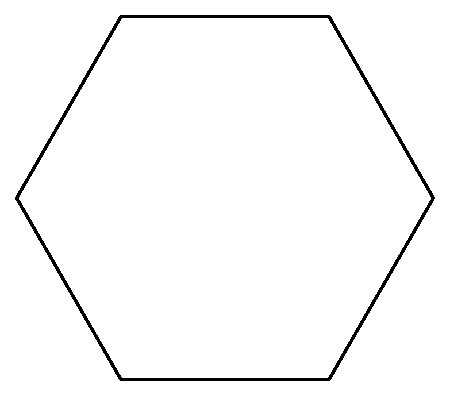
\includegraphics[width=4cm]{loopHexagon}}\label{exo:hexagonRepeat}
Draw a hexagon using the command \timesRepeat.
\end{exofigwithsize}


\newcommand{\replace}[2]{If}{When} you get the hang of it, try \newcommand{\replace}[2]{to augment}{increasing} the number of sides of a
polygon to a very large number. You may need to reduce the \newcommand{\replace}[2]{size}{length} of
the sides so \newcommand{\replace}[2]{that}{the} figure fits within the screen. When the
number of sides is large and the size of the sides is small, the
polygon will look like a circle.


\section{Pyramids Rediscovered}\label{sec:bouclonpyramids}
Remember how you coded the outline of the pyramid of Saqqarah in
\exoref{exo:saqqarah}? You can simplify your drawing by using a loop 
as follows:

\begin{scriptfig}{loopPyramid}{Pyramid script} \label{scr:pyramid}
| \caro |
\caro := \Turtle new.
5 timesRepeat: 
     [\caro north.
     \caro go: 20.
     \caro east.
     \caro go: 20].
5 timesRepeat: 
     [\caro go: 20.
     \caro south.
     \caro go: 20.
     \caro east].
\caro west.
\caro go: 200.
\end{scriptfig}

Now you \newcommand{\replace}[2]{should be able to}{can} generate pyramids with any number of
terraces \emph{with the same number of expressions}, just by changing
the numbers of the script.

\begin{exofig}{loopPyramid10} \label{exo:pyramid}
Try to draw a pyramid with 10 terraces using a variation of Script~\ref{scr:pyramid}.
\end{exofig}

You may want to generate pyramids with an even larger number of
terraces. The size of the terraces must be adjusted if you want
them to fit within the screen.

\section{Some Selected Problems}
As you have seen, the generation of the pyramid involves the
repetition of a block of code, which draws two line elements. Once the
proper repeating element is identified, one can produce complex
\newcommand{\replace}[2]{picture}{pictures} from elementary \newcommand{\replace}[2]{drawing}{drawings}, by \newcommand{\replace}[2]{repeating themselves}{repetition}.  The
following exercises illustrate this principle.

\begin{exofigwithsizeandtitle}{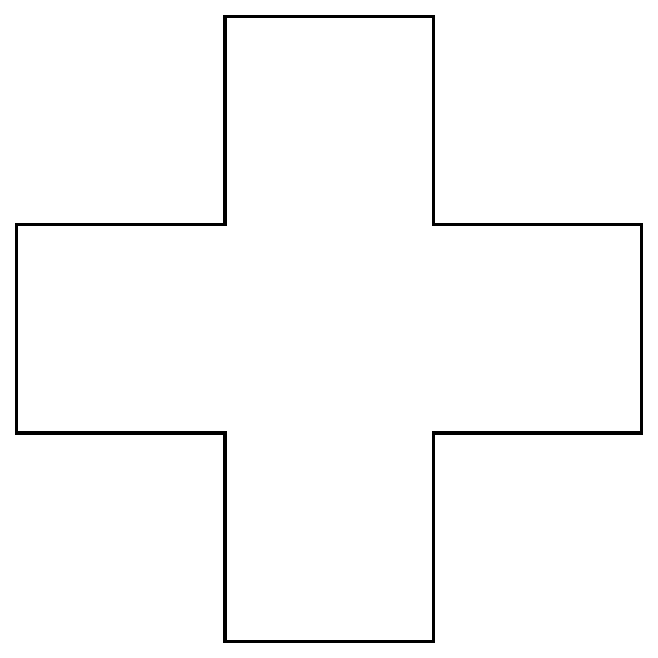
\includegraphics[width=4cm]{loopCross}}{Cross} \label{exo:redcross}
Draw the outline of the cross shown on the right using \turnLeft or \turnRight and
\timesRepeat.
\end{exofigwithsizeandtitle}


\begin{exofigwithtitle}{loopStair}{Stair}\label{exo:stair}
Draw the \newcommand{\replace}[2]{following stair}{stairway}.
\end{exofigwithtitle}


\hidden{| \caro |
\caro := \Turtle new.
10 timesRepeat: [ \caro go: 10.
                \caro north.
                \caro go: 10.
                \caro east]}

\begin{exofigwithtitle}{loopStylisedStair}{Stylized Stair}\label{exo:stylizedstair}
Draw \newcommand{\replace}[2]{the following}{this} stylized \newcommand{\replace}[2]{stair}{stairway}.
\end{exofigwithtitle}
\hidden{loopstylisedstair

	| \caro |
	\caro := \Turtle new.
	10 timesRepeat: [
                \caro go: 10.
                \caro north.
                \caro jump: 10.
                \caro east]}

\begin{exofigwithsizeandtitle}{
\includegraphics{loopSimpleElement}}{A Simple Element}\label{exo:element}
Draw the \newcommand{\remove}[1]{following} graphical element.
\end{exofigwithsizeandtitle}


\hidden{
| \caro |
\caro := \Turtle new.
\caro north. 
\caro go: 25.
\caro west.
\caro go: 25.
\caro south.
\caro go: 25}


\begin{exofigwithsizeandtitle}[0.3]{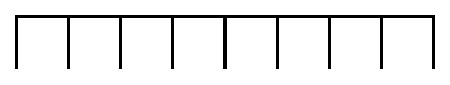
\includegraphics{loopComb}}{Comb}\label{exo:comb}
Transform \newcommand{\remove}[1]{the} \scriptref{exo:element} to produce a comb.
\end{exofigwithsizeandtitle}

\hidden{
| \caro |
\caro := \Turtle new.
8 timesRepeat: [\caro north. 
\caro go: 25.
\caro west.
\caro go: 25.
\caro south.
\caro go: 25]}


\begin{exofigwithsizeandtitle}{
\includegraphics{loopLadder}}{Ladder}\label{exo:ladder}
Transform \newcommand{\remove}[1]{the} \scriptref{exo:element} to produce a ladder.
\end{exofigwithsizeandtitle}


\hidden{
| \caro |
\caro := \Turtle new.
8 timesRepeat: [\caro north. 
\caro go: 25.
\caro west.
\caro go: 25.
\caro south.
\caro go: 25.
\caro north.
\caro jump: 25.
\caro east.
\caro jump: 25]}


\begin{exonofig}
Now that you \newcommand{\replace}[2]{master}{have mastered} loops\newcommand{\add}[1]{,} define a loop that draws the tumbling squares of the picture shown at the opening of Chapter~\ref{ch:relativeTurn}.
\end{exonofig}




\summa

\begin{table}[h]
\centering
\begin{tabular}{||p{6cm}|p{4cm}|p{4cm}||} \hline
% after \\ : \hline or \cline{col1-col2} \cline{col3-col4} ...
Method&Description&Example\\[1ex] \hline
\begin{nalltt}
n \timesRepeat
   \ct{[} a sequence of messages \ct{]}
\end{nalltt}
     &repeats \newcommand{\remove}[1]{\emph{n} times} a sequence of messages \newcommand{\add}[1]{\emph{n} times}
&\begin{nalltt}
10 timesRepeat: 
    [\caro go: 10. 
    \caro jump: 10]\end{nalltt} \\ \hline
\end{tabular}
\end{table}



\ifx\wholebook\relax\else\end{document}\fi

